\documentclass{report}

\input{preamble}
\input{macros}
\input{letterfonts}

\title{\Huge{Math 244}}
\author{\huge{PSET 1}}
\date{JAN 24 2025}

\begin{document}

\maketitle
\newpage% or \cleardoublepage
% \pdfbookmark[<level>]{<title>}{<dest>}
\pdfbookmark[section]{\contentsname}{toc}
\tableofcontents
\pagebreak

\section*{Section 1.2 Problem 5}
\addcontentsline{toc}{section}{Problem 5}

\qs{Section 1.2 Problem 5}{
    Is a "cancellation" possible for the Cartesion Product? That is,
    if $X \times Y = X \times Z$ holds for some sets, $X$, $Y$, and $Z$, does it follow that $Y = Z$? 
}

\begin{RemarkWithLily}{What is the Cartesian Product?}
    TThe Cartesian product of $X$ and $Y$ is the set of all ordered pairs of the form $(x,y)$, where $x \in X$ and $y \in Y$. 
\end{RemarkWithLily}

\begin{RemarkWithLily}{Asnwer}
    TThe "cancellation" is not possible for the Cartesian Product unless it is stated that $X$ is not an empty set. For if $X$ is an empty set, then the Cartesian Product of $X$ and 
    another set would always be the empty set. In this scenario, $Y$ and $Z$ could be different and their Cartesian Products with $X$ would still be the empty set.
\end{RemarkWithLily}

\section*{Section 1.2 Problem 6}
\addcontentsline{toc}{section}{Problem 6}

\qs{Section 1.2 Problem 6}{
    Prove that for any two sets $A$, $B$ we have 
    \begin{center}
        \[ \left(A \setminus B\right) \cup \left(B \setminus A \right) = \left( A \cup B \right) \setminus \left( A \cap B \right)\] 
    \end{center}
}

\begin{center}
    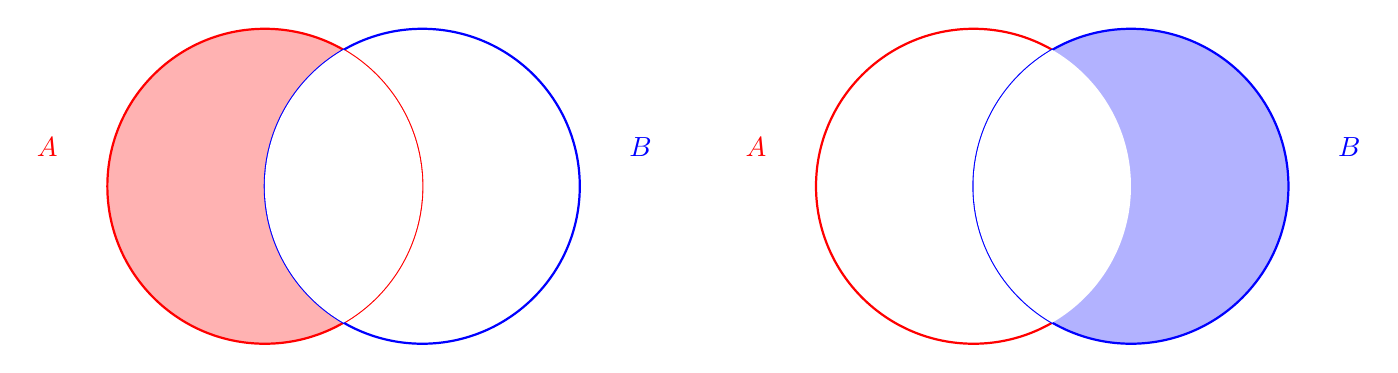
\begin{tikzpicture}
      \begin{scope}[shift={(-4,0)}]
        \filldraw[
          line width=0.8pt,
          color=red,
          fill=red!30
        ] (0,0) circle[radius=2cm]
          node[left=2.5cm, yshift=0.5cm] {\( A \)};
        
        \filldraw[
          line width=0.8pt,
          color=blue,
          fill=none
        ] (2,0) circle[radius=2cm]
          node[right=2.5cm, yshift=0.5cm] {\( B \)};
    
        \begin{scope}
          \clip (2,0) circle [radius=2cm]; 
          \fill[white] (0,0) circle [radius=2cm]; 
        \end{scope}
      \end{scope}
    
      \begin{scope}[shift={(5,0)}]
        \filldraw[
          line width=0.8pt,
          color=red,
          fill=none
        ] (0,0) circle[radius=2cm]
          node[left=2.5cm, yshift=0.5cm] {\( A \)};
        
        \filldraw[
          line width=0.8pt,
          color=blue,
          fill=blue!30
        ] (2,0) circle[radius=2cm]
          node[right=2.5cm, yshift=0.5cm] {\( B \)};
    
        \begin{scope}
          \clip (0,0) circle [radius=2cm]; 
          \fill[white] (2,0) circle [radius=2cm]; 
        \end{scope}
      \end{scope}
    \end{tikzpicture}
\end{center}

\begin{center}
    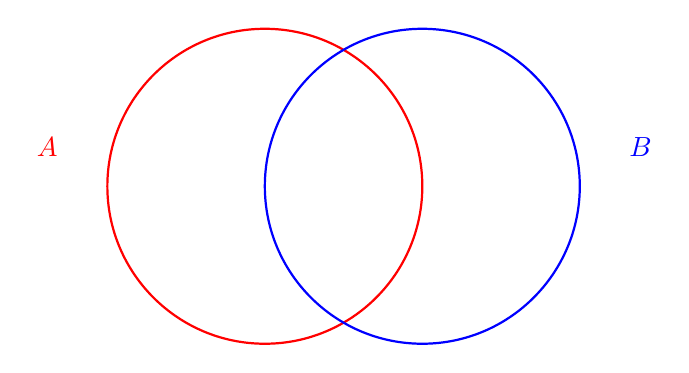
\begin{tikzpicture}
            \filldraw[
              line width=0.8pt,
              color=red,
              fill= none
            ] (0,0) circle[radius=2cm]
              node[left=2.5cm, yshift=0.5cm] {\( A \)};
            
            \filldraw[
              line width=0.8pt,
              color=blue,
              fill= none
            ] (2,0) circle[radius=2cm]
              node[right=2.5cm, yshift=0.5cm] {\( B \)};
    \end{tikzpicture}
\end{center}
    
\begin{center}
    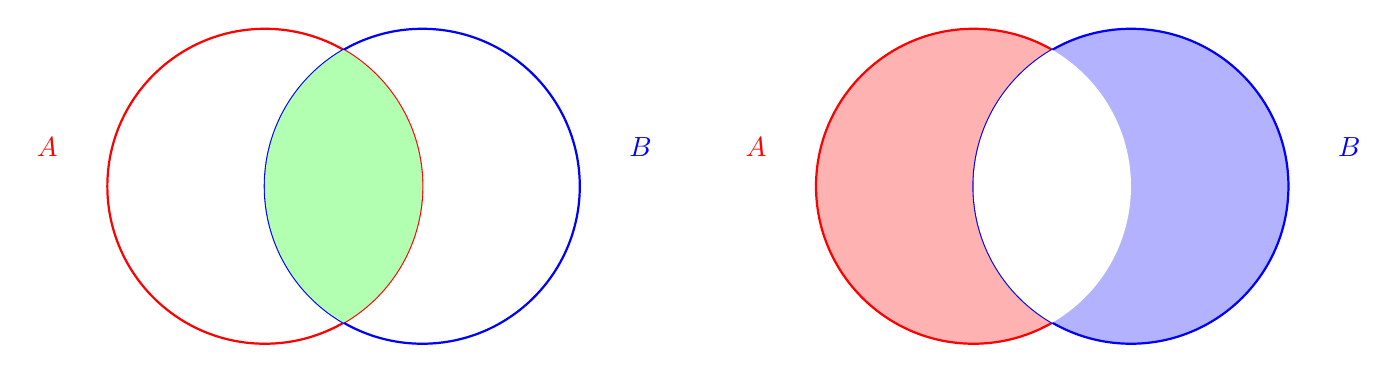
\begin{tikzpicture}
        \begin{scope}[shift={(-4,0)}]
            \filldraw[
              line width=0.8pt,
              color=red,
              fill= none
            ] (0,0) circle[radius=2cm]
              node[left=2.5cm, yshift=0.5cm] {\( A \)};
            
            \filldraw[
              line width=0.8pt,
              color=blue,
              fill= none
            ] (2,0) circle[radius=2cm]
              node[right=2.5cm, yshift=0.5cm] {\( B \)};
            
            \begin{scope}
                \clip (0,0) circle [radius=2cm]; 
                \fill[green!30] (2,0) circle [radius=2cm]; 
            \end{scope}
        \end{scope}

        \begin{scope}[shift={(5,0)}]
            \filldraw[
              line width=0.8pt,
              color=red,
              fill= red!30
            ] (0,0) circle[radius=2cm]
              node[left=2.5cm, yshift=0.5cm] {\( A \)};
            
            \filldraw[
              line width=0.8pt,
              color= blue,
              fill= blue!30
            ] (2,0) circle[radius=2cm]
              node[right=2.5cm, yshift=0.5cm] {\( B \)};
            
            \begin{scope}
                \clip (0,0) circle [radius=2cm]; 
                \fill[white] (2,0) circle [radius=2cm]; 
            \end{scope}
        \end{scope}

    \end{tikzpicture}
\end{center}

\section*{Section 1.3 Problem 2}
\addcontentsline{toc}{section}{Problem 2}

\qs{Section 1.3 Problem 2}{
    The numbers $F_{0}$, $F_{1}$, $F_{2}$, $F_{3}$, $\ldots$ are defined as follows:
        \begin{center}
            \[ F_{0} = 0, F_{1} = 1, F_{n+2} = F_{n+1} + F_{n} \text{for } n = 0,1,2, \ldots \] 
        \end{center}
    Prove that for any $n \geq 0$ we have $F_{n} \leq \left(\frac{1 + \sqrt{5}}{2}\right)^{n-1}$
}

\section*{1.4 Problem 2}
\addcontentsline{toc}{section}{Problem 2}

\qs{Section 1.4 Problem 2}{
    Find an example of: 
    \begin{enumerate}
        \item[(a)] A one-to-one function $f: \mathbb{N} \to \mathbb{N}$ that is not onto.
        \item[(b)] A function $f: \mathbb{N} \to \mathbb{N}$ that is onto but not one-to-one. 
    \end{enumerate}
}

\section*{1.4 Problem 6}
\addcontentsline{toc}{section}{Problem 6}

\qs{}{
    Prove that the following two statements about a function $g_{1}$ : $Z \to X$ and $g_{2}$ : $Z \to X$ 
    the composed functions $f \circ g_{1}$ and $f \circ g_{2}$ are also distinct.
}

\end{document}